\documentclass{article}
\usepackage{graphicx}
\usepackage{color}
\usepackage[english]{babel}
\usepackage[utf8]{inputenc}
\usepackage[color]{vdmlisting}
\usepackage[hidelinks]{hyperref} 
\usepackage{longtable}
\usepackage{lscape}
\usepackage{rotating}

\begin{document}
\title{\Huge\textbf{\textit{Electronic Voting System}}\linebreak
\Large\textbf{\\Assignment 5 (T05)}\linebreak\linebreak\linebreak

\includegraphics[width=8cm]{feup.pdf}\linebreak \linebreak
\large{Mestrado Integrado em Engenharia Informática e Computação} \linebreak
\large{Métodos Formais em Engenharia de \textit{Software}  \\ EIC0039-1S}\linebreak
}
\author{\\\\\\\\\\\\\\\\\\\
João de Sá Balão Calisto Correia - 201208114 (ei12159@fe.up.pt)\\
João Pedro Matos Teixeira Dias - 201106781 (ei11137@fe.up.pt)\\
Eduardo José Valadar Martins  - 201104191 (ei11104@fe.up.pt)\\
\\ Faculdade de Engenharia da Universidade do Porto \\ Rua Roberto Frias, s\/n, 4200-465 Porto, Portugal
 \vspace{1cm}}
%\date{Junho de 2007}

\maketitle
\newpage
\tableofcontents
\newpage
\section{Informal system description and list of requirements}
\subsection{Informal system description}
\subsection{Requirements List}

\begin{center}
    \begin{tabular}{ | l | l  | p{9cm} |}
    \hline
    ID	& Priority & Description \\ \hline
    R1 &	Mandatory&	The Voter can start voting by indicating his name and code. \\ \hline
   R2& Mandatory&The Voter can choose candidate from ballot by indicating his name.\\ \hline
    R3	&Mandatory&	The Vote Table can create/manage an election adding it a new Voter or a new Candidate. \\ \hline
  R4&Mandatory&The Vote Table, after the voting action from Voter, should be able to remove from the list that Voter, using his name and code.  \\ 
    \hline
    \end{tabular}
\end{center}

\section{Visual UML Model}
\subsection{Use case model}

\begin{center}
    \begin{tabular}{ | l | p{9cm} |}
    \hline
   \textbf{Scenario}	& \textbf{Starting Vote}  \\ \hline
    \textbf{Description}	& Normal scenario for initialize the vote act and for update the current voter. \\ \hline
   \textbf{Pre-conditions}	& 1.The current state of State Machine is STOP.\linebreak
2.The voters of the PEB are not empty.\linebreak
3.The current voter is in voters of PEB. (\textit{input})\linebreak
4.The current voter is not in voters of PEB. (\textit{input})
\\ \hline
 \textbf{Post-conditions} &	1.	The current State of State Machine is INIT. (\textit{final system state})\linebreak
2.	The Voter is the same voter in the ballot. (\textit{final system state})
   \\ \hline
   \textbf{Steps} &	(unspecified) \\ 
    \hline
\textbf{Exceptions}& 	(unspecified)
 \\ 
    \hline
    \end{tabular}
\end{center}

\begin{center}
    \begin{tabular}{ | l | p{9cm} |}
    \hline
   \textbf{Scenario}	& \textbf{Choose candidate from ballot}  \\ \hline
    \textbf{Description}	& Normal scenario for choosing a candidate from a list of them. \\ \hline
   \textbf{Pre-conditions}	& 1.The current state of State Machine is INIT.\linebreak
2.The current voter is in PEB voters.\linebreak
3.The candidate exists in the ballot.
 (\textit{input})
\\ \hline
 \textbf{Post-conditions} &1.The current State of State Machine is CONFIRM. (\textit{final system state})\linebreak
2.The voted candidate is the same that the selected in ballot. (\textit{final system state})\linebreak
3.The current voter is in PEB voters. (\textit{final system state})\linebreak
4.The current candidate is in PEB ballot. (\textit{final system state})

   \\ \hline
   \textbf{Steps} &	(unspecified) \\ 
    \hline
\textbf{Exceptions}& 	(unspecified)
 \\ 
    \hline
    \end{tabular}
\end{center}


\begin{center}
    \begin{tabular}{ | l | p{9cm} |}
    \hline
   \textbf{Scenario}	& \textbf{Confirm Vote}  \\ \hline
    \textbf{Description}	& Normal scenario for choosing a candidate from a list of them.\\ \hline
   \textbf{Pre-conditions}	& 1.The current state of State Machine is confirm.\linebreak
2.The Voter name exists.\linebreak
3.The Candidate name exists.

\\ \hline
 \textbf{Post-conditions} & 1.The current State of State Machine is STOP. (\textit{final system state})\linebreak
2.The current voter is in PEB previous voters. (\textit{final system state})\linebreak
3.The current voter is not in PEB voters. (\textit{final system state})\linebreak
Or\linebreak
1.The current State of State Machine is INIT. (\textit{final system state})\linebreak
2.The current voter is in PEB voters. (\textit{final system state})\linebreak
Or\linebreak
1.The current State of State Machine is END. (\textit{final system state})\linebreak
2.The current voter is in PEB previous voters. (\textit{final system state})\linebreak
3.The current voter is not in PEB voters. (\textit{final system state})
   \\ \hline
   \textbf{Steps} &1.The Voter chooses a candidate.\linebreak
2.The Voter confirm is vote.
 \\ 
    \hline
\textbf{Exceptions}& 	(unspecified)
 \\ 
    \hline
    \end{tabular}
\end{center}

\begin{center}
    \begin{tabular}{ | l | p{9cm} |}
    \hline
   \textbf{Scenario}	& \textbf{Add new Voter }  \\ \hline
    \textbf{Description}	&Normal scenario for adding a Voter to PEB.\\ \hline
   \textbf{Pre-conditions}	&1.The Voter name is not empty.\linebreak
2.The Voter code is valid (between 1000 and 9999).
\\ \hline
 \textbf{Post-conditions} & 1.The Voter is added to PEB as intended. (\textit{final system state}) \\ \hline
   \textbf{Steps} &  (unspecified)
 \\ 
    \hline
\textbf{Exceptions}& 	(unspecified)
 \\ 
    \hline
    \end{tabular}
\end{center}

\begin{center}
    \begin{tabular}{ | l | p{9cm} |}
    \hline
   \textbf{Scenario}	& \textbf{Add new Candidate }  \\ \hline
    \textbf{Description}	&Normal scenario for adding a Candidate to PEB.\\ \hline
   \textbf{Pre-conditions}	&1.The Candidate name is not empty.
\\ \hline
 \textbf{Post-conditions} & 1.The Candidate is added to PEB as intended. (final system state)  (\textit{final system state}) \\ \hline
   \textbf{Steps} &  (unspecified)
 \\ 
    \hline
\textbf{Exceptions}& 	(unspecified)
 \\ 
    \hline
    \end{tabular}
\end{center}

\begin{figure}[!h]
\centering
	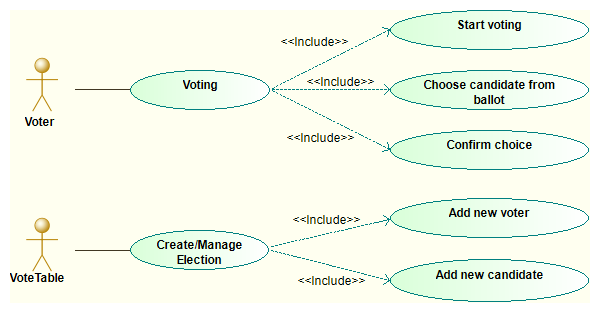
\includegraphics[width=\textwidth,height=\textheight,keepaspectratio]{use.png}
	\caption{Use Case Diagram.}
	\label{fig:PropProf}
\end{figure}
\subsection{State machine model}
\begin{figure}[h!]
\centering
	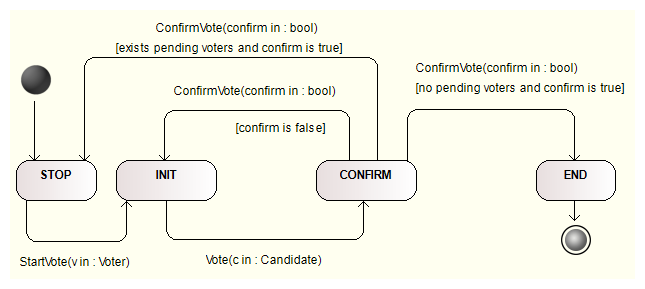
\includegraphics[width=\textwidth,height=\textheight,keepaspectratio]{state.png}
	\caption{State Machine Diagram (Vote Process).}
	\label{fig:PropProf}
\end{figure}
\subsection{Class model}
\begin{figure}[!h]
\centering
	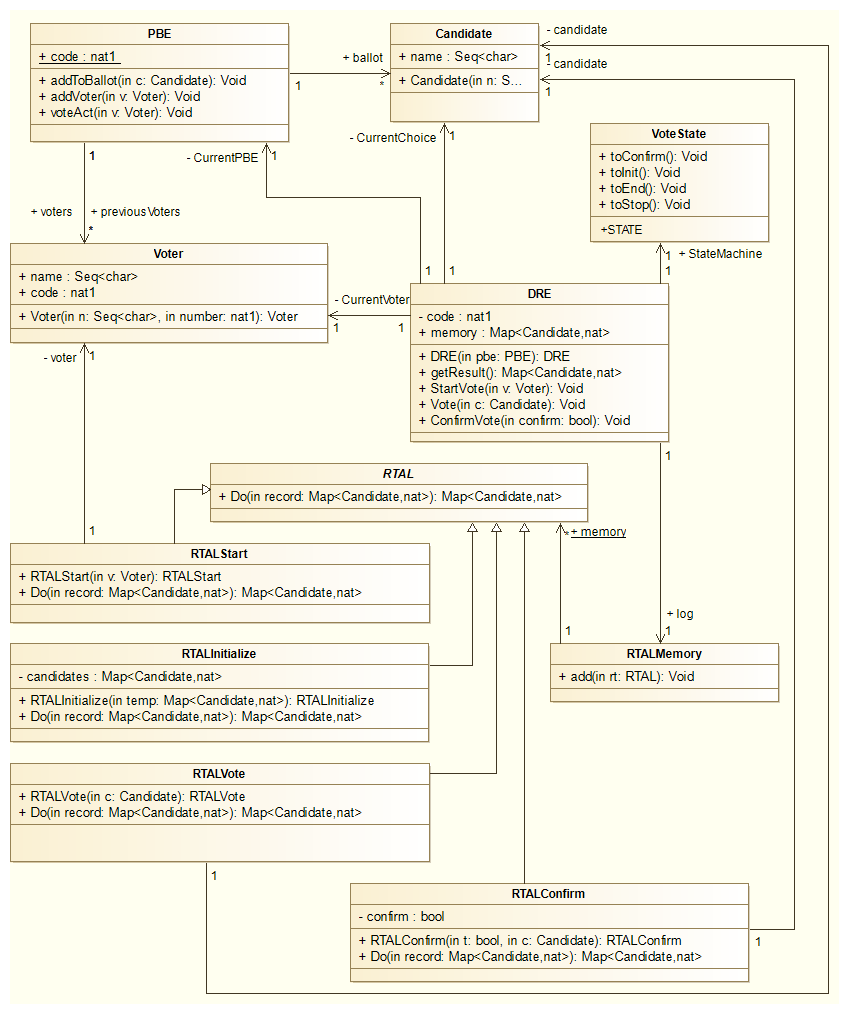
\includegraphics[width=\textwidth,height=\textheight,keepaspectratio]{uml.png}
	\caption{Class Model Diagram.}
	\label{fig:PropProf}
\end{figure}
\section{Formal VDM++ Model}\label{xpto}
\subsection{Candidate}
\begin{vdmpp}
class Candidate
instance variables
 public name: seq of char;
operations
--Constructor-Create a new Candidate
(*@
\label{Candidate:6}
@*)
 public Candidate: seq of char ==> Candidate
 Candidate(n) == (name := n; return self)
 pre name <> []
 post name = n
end Candidate
\end{vdmpp}
\bigskip
\begin{longtable}{|l|r|r|r|}
\hline
Function or operation & Line & Coverage & Calls \\
\hline
\hline
\hyperref[Candidate:6]{Candidate} & 6&100.0\% & 140 \\
\hline
\hline
Candidate.vdmpp & & 100.0\% & 140 \\
\hline
\end{longtable}


\subsection{Voter}
\begin{vdmpp}
class Voter
instance variables
 public name: seq of char;
 public code: nat1;
operations
--Constructor-Create a new Voter
(*@
\label{Voter:7}
@*)
 public Voter: seq of char * nat1 ==> Voter
 Voter(n,number) == (name := n;
           code:=number; 
           return self)
 pre 
  name <> [] and
  number >= 1000 and
  number <= 9999
 post 
  name = n and
  code = number
end Voter
\end{vdmpp}
\bigskip
\begin{longtable}{|l|r|r|r|}
\hline
Function or operation & Line & Coverage & Calls \\
\hline
\hline
\hyperref[Voter:7]{Voter} & 7&100.0\% & 140 \\
\hline
\hline
Voter.vdmpp & & 100.0\% & 140 \\
\hline
\end{longtable}


\subsection{PBE}
\begin{vdmpp}
class PBE
instance variables
 public ballot: set of Candidate := {};
 public voters: set of Voter := {};
 public previousVoters:  set of Voter :={};
 public static code: nat1 :=9999;
 --inv cannot exists the same vouter in previousVoters and vice-versa
 inv card (voters inter previousVoters) = 0;
operations
--Add new Candidate to PBE ballot set
(*@
\label{addToBallot:11}
@*)
 public addToBallot: Candidate ==> ()
 addToBallot(c) == ballot := {c} union ballot
 pre c.name <> []
 post c in set ballot;
--Add new Voter to PBE voters set
  public addVoter: Voter ==> ()
(*@
\label{addVoter:17}
@*)
 addVoter(v) == voters := {v} union voters
 pre v.name <> []
  and v.code > 1000 
  and v.code < 9999
 post v in set voters;
 
--Voter finished
 public voteAct: Voter ==> ()
(*@
\label{voteAct:25}
@*)
 voteAct(v) == (
         voters := remove[Voter](v,voters);
         previousVoters := previousVoters union {v}
        )
 pre v in set voters
 post v in set previousVoters
    and v not in set voters
    and card voters = card voters~-1
    and card previousVoters = card previousVoters~+1;
functions
    public remove[@T](e: @T, s: set of @T) res: set of @T ==
(*@
\label{remove:36}
@*)
     {x | x in set s & x <> e};
end PBE
\end{vdmpp}
\bigskip
\begin{longtable}{|l|r|r|r|}
\hline
Function or operation & Line & Coverage & Calls \\
\hline
\hline
\hyperref[addToBallot:11]{addToBallot} & 11&100.0\% & 140 \\
\hline
\hyperref[addVoter:17]{addVoter} & 17&100.0\% & 40 \\
\hline
\hyperref[remove:36]{remove} & 36&100.0\% & 25 \\
\hline
\hyperref[voteAct:25]{voteAct} & 25&100.0\% & 25 \\
\hline
\hline
PBE.vdmpp & & 100.0\% & 230 \\
\hline
\end{longtable}


\subsection{VoteState}
\begin{vdmpp}
class VoteState
types
 public STATE = <INIT> | <CONFIRM> | <STOP> | <END>;
instance variables
 public currentState: STATE := <STOP>;
operations
(*@
\label{toConfirm:7}
@*)
 public toConfirm: () ==> ()
 toConfirm() == currentState := <CONFIRM>
 pre currentState = <INIT>
 post currentState = <CONFIRM>;
 
(*@
\label{toInit:12}
@*)
 public toInit: () ==> ()
 toInit() == currentState := <INIT>
 pre currentState = <STOP> or  currentState = <CONFIRM>
 post currentState = <INIT>;
 
(*@
\label{toEnd:17}
@*)
 public toEnd: () ==> ()
 toEnd() == currentState := <END>
 pre currentState = <CONFIRM>
 post currentState = <END>;
 
(*@
\label{toStop:22}
@*)
 public toStop: () ==> ()
 toStop() == currentState := <STOP>
 post currentState = <STOP>;
end VoteState
\end{vdmpp}
\bigskip
\begin{longtable}{|l|r|r|r|}
\hline
Function or operation & Line & Coverage & Calls \\
\hline
\hline
\hyperref[toConfirm:7]{toConfirm} & 7&100.0\% & 94 \\
\hline
\hyperref[toEnd:17]{toEnd} & 17&100.0\% & 14 \\
\hline
\hyperref[toInit:12]{toInit} & 12&100.0\% & 96 \\
\hline
\hyperref[toStop:22]{toStop} & 22&100.0\% & 106 \\
\hline
\hline
VoteState.vdmpp & & 100.0\% & 310 \\
\hline
\end{longtable}


\subsection{DRE}
\begin{vdmpp}
class DRE
instance variables
 private code: nat1 :=9999;
 private memory: map Candidate to nat := {|->} ;
 public log: RTALMemory := new RTALMemory();
 private CurrentPBE: PBE;
 public StateMachine: VoteState := new VoteState();
 private CurrentChoice: Candidate := new Candidate(); 
 private CurrentVoter: Voter := new Voter();
 
 inv card CurrentPBE.ballot > 0;
operations
-- Constructor
(*@
\label{DRE:14}
@*)
 public DRE: PBE ==> DRE 
 DRE(pbe) == (
       
       CurrentPBE := pbe;
       StateMachine.toStop();
       memory :={|->};
       for all cand in set CurrentPBE.ballot do
          (
        memory:=memory++{cand|->0};
          );
          log.add(new RTALInitialize(memory));
       return self)
 pre 
  pbe.ballot <> {}
  and pbe.voters <> {}
  and pbe.code = code
 post 
  self.CurrentPBE.ballot = pbe.ballot
  and self.CurrentPBE.voters = pbe.voters;
 
(*@
\label{getResult:34}
@*)
 public getResult:() ==> map Candidate to nat
 getResult()== return memory;
 
--Voting sequence state machine
(*@
\label{StartVote:38}
@*)
 public StartVote: Voter ==> ()
 StartVote(v) == (
   log.add(new RTALStart(v));
   StateMachine.toInit();
   CurrentVoter := v;
 )
 pre StateMachine.currentState=<STOP>
   and card CurrentPBE.voters <> 0
   and v in set CurrentPBE.voters
   and v not in set CurrentPBE.previousVoters
 post StateMachine.currentState=<INIT>
    and v = CurrentVoter;

(*@
\label{Vote:51}
@*)
 public Vote: Candidate ==> ()
 Vote(c) == (
   log.add(new RTALVote(c));
   StateMachine.toConfirm();
   CurrentChoice := c
 )
 pre StateMachine.currentState=<INIT>
   and CurrentVoter in set CurrentPBE.voters
   and c in set CurrentPBE.ballot
 post StateMachine.currentState=<CONFIRM>
    and c = CurrentChoice
    and CurrentVoter in set CurrentPBE.voters
    and CurrentChoice in set CurrentPBE.ballot;
 ------------------------------------------------------------------------------------
(*@
\label{ConfirmVote:65}
@*)
 public ConfirmVote: bool ==>()
 ConfirmVote(confirm) == (
   log.add(new RTALConfirm(confirm,CurrentChoice));
   if(confirm)
   then(
     memory(CurrentChoice):=memory(CurrentChoice)+1;
     CurrentPBE.voteAct(CurrentVoter); 
     if(CurrentPBE.voters = {})
     then(
      StateMachine.toEnd();
     )
     else(
      StateMachine.toStop();
     );
     )
   else(
     StateMachine.toInit();
     )
 )
 pre StateMachine.currentState=<CONFIRM> 
   and CurrentVoter.name <> []
   and CurrentChoice.name <> []
 post (StateMachine.currentState=<STOP>
    and CurrentVoter in set CurrentPBE.previousVoters
    and CurrentVoter not in set CurrentPBE.voters
    )
    or (
    StateMachine.currentState=<INIT>
    and CurrentVoter in set CurrentPBE.voters)
    or (
    StateMachine.currentState=<END>
    and CurrentVoter in set CurrentPBE.previousVoters
    and CurrentVoter not in set CurrentPBE.voters
    );
functions
 
end DRE
\end{vdmpp}
\bigskip
\begin{longtable}{|l|r|r|r|}
\hline
Function or operation & Line & Coverage & Calls \\
\hline
\hline
\hyperref[ConfirmVote:65]{ConfirmVote} & 65&100.0\% & 24 \\
\hline
\hyperref[DRE:14]{DRE} & 14&100.0\% & 9 \\
\hline
\hyperref[StartVote:38]{StartVote} & 38&100.0\% & 21 \\
\hline
\hyperref[Vote:51]{Vote} & 51&100.0\% & 24 \\
\hline
\hyperref[getResult:34]{getResult} & 34&100.0\% & 15 \\
\hline
\hline
DRE.vdmpp & & 100.0\% & 93 \\
\hline
\end{longtable}


\subsection{RTAL}
\begin{vdmpp}
class RTALMemory
instance variables
  public static memory: seq of RTAL := [];
operations
 public add: RTAL ==> ()
(*@
\label{add:6}
@*)
 add(rt)==(
  memory := memory ^ [rt]; 
 )
 post len memory = len memory~+1;
end RTALMemory
-----------------------------------------------------------------------
(*@
\label{RTALMemory:12}
@*)
class RTAL 
instance variables
operations
 public Do : (map Candidate to nat) ==> (map Candidate to nat)
 Do(record) == is subclass responsibility;
end RTAL
----------------------------------------------------------------------
class RTALInitialize is subclass of RTAL
instance variables
 candidates : map Candidate to nat;
operations
 public RTALInitialize: map Candidate to nat ==> RTALInitialize 
(*@
\label{Do:24}
@*)
 RTALInitialize(temp) == (
       candidates := temp;
       return self)
 pre card dom temp <> 0
 post candidates = temp;
 
 public Do :  (map Candidate to nat) ==> (map Candidate to nat)
 Do(record) ==  (
(*@
\label{RTALStart:32}
@*)
(*@
\label{RTALStart:32}
@*)
(*@
\label{RTALInitialize:32}
@*)
  dcl temp : map Candidate to nat := record;
  temp :=candidates;
  return temp)
 pre card dom candidates <> 0;
 
end RTALInitialize

(*@
\label{Do:39}
@*)
(*@
\label{Do:39}
@*)
----------------------------------------------------------------------

class RTALStart is subclass of RTAL
instance variables
 voter : Voter;
operations
 public RTALStart: Voter ==> RTALStart 
 RTALStart(v) == (
       voter := v;
       return self)
(*@
\label{RTALVote:49}
@*)
 pre v.name <> []
 post voter = v;
 
 public Do :  (map Candidate to nat) ==> (map Candidate to nat)
 Do(record) ==  (return record;)
 pre voter.name <> [];
 
(*@
\label{Do:56}
@*)
end RTALStart
--------------------------------------------------------------
class RTALVote is subclass of RTAL
instance variables
  candidate : Candidate;
operations
 public RTALVote: Candidate ==> RTALVote 
 RTALVote(c) == (
       candidate := c;
       return self);
(*@
\label{RTALConfirm:66}
@*)
 
 public Do :  (map Candidate to nat) ==> (map Candidate to nat)
 Do(record) == (return record;)
 pre candidate.name <> [];
end RTALVote
----------------------------------------------------------------
class RTALConfirm is subclass of RTAL
(*@
\label{Do:73}
@*)
instance variables 
 confirm : bool := false;
 candidate : Candidate;
operations
 public RTALConfirm: bool*Candidate ==> RTALConfirm 
 RTALConfirm(t,c) == (
       confirm := t;
       candidate:= c;
       return self)
 post confirm = t;

 public Do : (map Candidate to nat) ==> (map Candidate to nat)
 Do(record) == (
  dcl temp:map Candidate to nat := record;
  if(confirm)
  then(
   temp(candidate):=temp(candidate)+1;
   return temp;
  )
  else(
   return temp;
  );
 )
 pre (confirm = true or confirm = false)
end RTALConfirm

\end{vdmpp}
\bigskip
\begin{longtable}{|l|r|r|r|}
\hline
Function or operation & Line & Coverage & Calls \\
\hline
\hline
\hyperref[Do:73]{Do} & 73&100.0\% & 37 \\
\hline
\hyperref[Do:56]{Do} & 56&100.0\% & 37 \\
\hline
\hyperref[Do:39]{Do} & 39&100.0\% & 13 \\
\hline
\hyperref[Do:39]{Do} & 39&100.0\% & 52 \\
\hline
\hyperref[Do:24]{Do} & 24&100.0\% & 5 \\
\hline
\hyperref[RTALConfirm:66]{RTALConfirm} & 66&100.0\% & 20 \\
\hline
\hyperref[RTALInitialize:32]{RTALInitialize} & 32&100.0\% & 10 \\
\hline
\hyperref[RTALMemory:12]{RTALMemory} & 12&100.0\% & 5 \\
\hline
\hyperref[RTALStart:32]{RTALStart} & 32&100.0\% & 13 \\
\hline
\hyperref[RTALStart:32]{RTALStart} & 32&100.0\% & 18 \\
\hline
\hyperref[RTALVote:49]{RTALVote} & 49&100.0\% & 20 \\
\hline
\hyperref[add:6]{add} & 6&100.0\% & 91 \\
\hline
\hline
RTAL.vdmpp & & 100.0\% & 321 \\
\hline
\end{longtable}


\section{Model Validation}
\subsection{EVSTestSuit}
\begin{vdmpp}
class EVSTestSuit

instance variables
 voteTable: PBE := new PBE();
 voterOne: Voter := new Voter("Joaquim",1001);
 voterTwo: Voter :=  new Voter("Joao",1002);
 voterThree: Voter:= new Voter("Correia",1003);
 voterFour: Voter:= new Voter("Rui",1004);
 candidateOne: Candidate:= new Candidate("PS");
 candidateTwo: Candidate:= new Candidate("PSD");
 candidateThree: Candidate:= new Candidate("CDS");
 candidateFour: Candidate:= new Candidate("Livre");
 VotingProcess: DRE := new DRE();
operations

(*@
\label{assertTrue:16}
@*)
private assertTrue: bool ==> ()
 assertTrue(cond) == return
 pre cond;

(*@
\label{testVoting:20}
@*)
private testVoting: () ==> ()
testVoting() ==
(
 dcl record: map Candidate to nat :={|->};
 
 voteTable.addVoter(voterOne);
 voteTable.addVoter(voterTwo);
 voteTable.addVoter(voterThree);
 voteTable.addVoter(voterFour);
 assertTrue(card voteTable.voters = 4);
 voteTable.addToBallot(candidateOne);
 voteTable.addToBallot(candidateTwo);
 voteTable.addToBallot(candidateThree);
 voteTable.addToBallot(candidateFour);
 assertTrue(card voteTable.ballot = 4);
 VotingProcess:= new DRE(voteTable);
 VotingProcess.StartVote(voterOne);
 VotingProcess.Vote(candidateOne);
 VotingProcess.ConfirmVote(true);
 assertTrue(card voteTable.voters = 3);
 assertTrue(card voteTable.previousVoters = 1);
 VotingProcess.StartVote(voterTwo);
 VotingProcess.Vote(candidateOne);
 VotingProcess.ConfirmVote(true);
 assertTrue(VotingProcess.getResult()(candidateOne)=2);
 assertTrue(card voteTable.voters = 2);
 assertTrue(card voteTable.previousVoters = 2);
 
 for entry in RTALMemory`memory 
  do (
    record:=entry.Do(record);
  );
  assertTrue(VotingProcess.memory = record);
  
);
(*@
\label{testReChoiceVoting:55}
@*)

private testReChoiceVoting: () ==> ()
testReChoiceVoting() ==
( 
 dcl record: map Candidate to nat:={|->};
 
 voteTable.addVoter(voterOne);
 voteTable.addVoter(voterTwo);
 voteTable.addVoter(voterThree);
 voteTable.addVoter(voterFour);
 assertTrue(card voteTable.voters = 4);
 voteTable.addToBallot(candidateOne);
 voteTable.addToBallot(candidateTwo);
 voteTable.addToBallot(candidateThree);
 voteTable.addToBallot(candidateFour);
 assertTrue(card voteTable.ballot = 4);
 VotingProcess:= new DRE(voteTable);
 VotingProcess.StartVote(voterOne);
 VotingProcess.Vote(candidateOne);
 VotingProcess.ConfirmVote(false);
 assertTrue(card voteTable.voters = 4);
 assertTrue(card voteTable.previousVoters = 0);
 VotingProcess.Vote(candidateTwo);
 VotingProcess.ConfirmVote(true);
 assertTrue(VotingProcess.getResult()(candidateTwo)=1);
 assertTrue(card voteTable.voters = 3);
 assertTrue(card voteTable.previousVoters = 1);
 
 for entry in RTALMemory`memory 
  do (
    record:=entry.Do(record);
  );
   
(*@
\label{testEnd:88}
@*)
  assertTrue(VotingProcess.memory = record);
);

private testEnd: () ==> ()
testEnd() ==
( 
 dcl record: map Candidate to nat:={|->};
 voteTable.addVoter(voterOne);
 voteTable.addVoter(voterTwo);
 voteTable.addVoter(voterThree);
 voteTable.addVoter(voterFour);
 assertTrue(card voteTable.voters = 4);
 voteTable.addToBallot(candidateOne);
 voteTable.addToBallot(candidateTwo);
 voteTable.addToBallot(candidateThree);
 voteTable.addToBallot(candidateFour);
 assertTrue(card voteTable.ballot = 4);
 VotingProcess:= new DRE(voteTable);
 VotingProcess.StartVote(voterOne);
 VotingProcess.Vote(candidateOne);
 VotingProcess.ConfirmVote(true);
 VotingProcess.StartVote(voterTwo);
 VotingProcess.Vote(candidateOne);
 VotingProcess.ConfirmVote(true);
 VotingProcess.StartVote(voterThree);
 VotingProcess.Vote(candidateTwo);
 VotingProcess.ConfirmVote(true);
 VotingProcess.StartVote(voterFour);
 VotingProcess.Vote(candidateTwo);
 VotingProcess.ConfirmVote(true);
 assertTrue(VotingProcess.StateMachine.currentState = <END>);
 
 --audit
 for entry in RTALMemory`memory 
  do (
    record:=entry.Do(record);
  );
(*@
\label{main:125}
@*)
   
  assertTrue(VotingProcess.memory = record);
);

public static main: () ==> ()
main() ==(
 new EVSTestSuit().testEnd();
 new EVSTestSuit().testVoting();
 new EVSTestSuit().testReChoiceVoting();
);

end EVSTestSuit
\end{vdmpp}
\bigskip
\begin{longtable}{|l|r|r|r|}
\hline
Function or operation & Line & Coverage & Calls \\
\hline
\hline
\hyperref[assertTrue:16]{assertTrue} & 16&100.0\% & 200 \\
\hline
\hyperref[main:125]{main} & 125&100.0\% & 4 \\
\hline
\hyperref[testEnd:88]{testEnd} & 88&100.0\% & 4 \\
\hline
\hyperref[testReChoiceVoting:55]{testReChoiceVoting} & 55&100.0\% & 3 \\
\hline
\hyperref[testVoting:20]{testVoting} & 20&100.0\% & 9 \\
\hline
\hline
EVSTestSuit.vdmpp & & 100.0\% & 220 \\
\hline
\end{longtable}


\renewcommand{\refname}{\section{Bibliography}} 
\begin{thebibliography}{99}
\bibitem{intro} 
Pipattanasomporn M., Feroze H. and Rahman S., Multi-agent systems in a distributed smart grid: Design and implementation, 2009.
\end{thebibliography}



\end{document}
